%versi 3 (22-07-2020)
\chapter{Analisis}
\label{chap:analisis}
Pada bab ini akan dijelaskan mengenai proses pengumpulan data citra satelit yang berada di Hadoop LAB Unpar, pengkonversian data \textit{text} menjadi gambar, dan bagaimana cara penggabungan gambar. Juga akan menjelaskan tetang analisis kebutuhan dalam perancangan perangkat lunak. 

\section{Proses Pembentukan Gambar}
Pada Gambar \ref{fig:ciumbuleuit} merupakan hasil dari penggabungan gambar per \textit{tile}. Langkah-langkah dalam proses pengambilan data berupa gambar citra satelit dari kecamatan atau kelurahan di Kota Bandung. 
\begin{figure}[H]
	\centering
	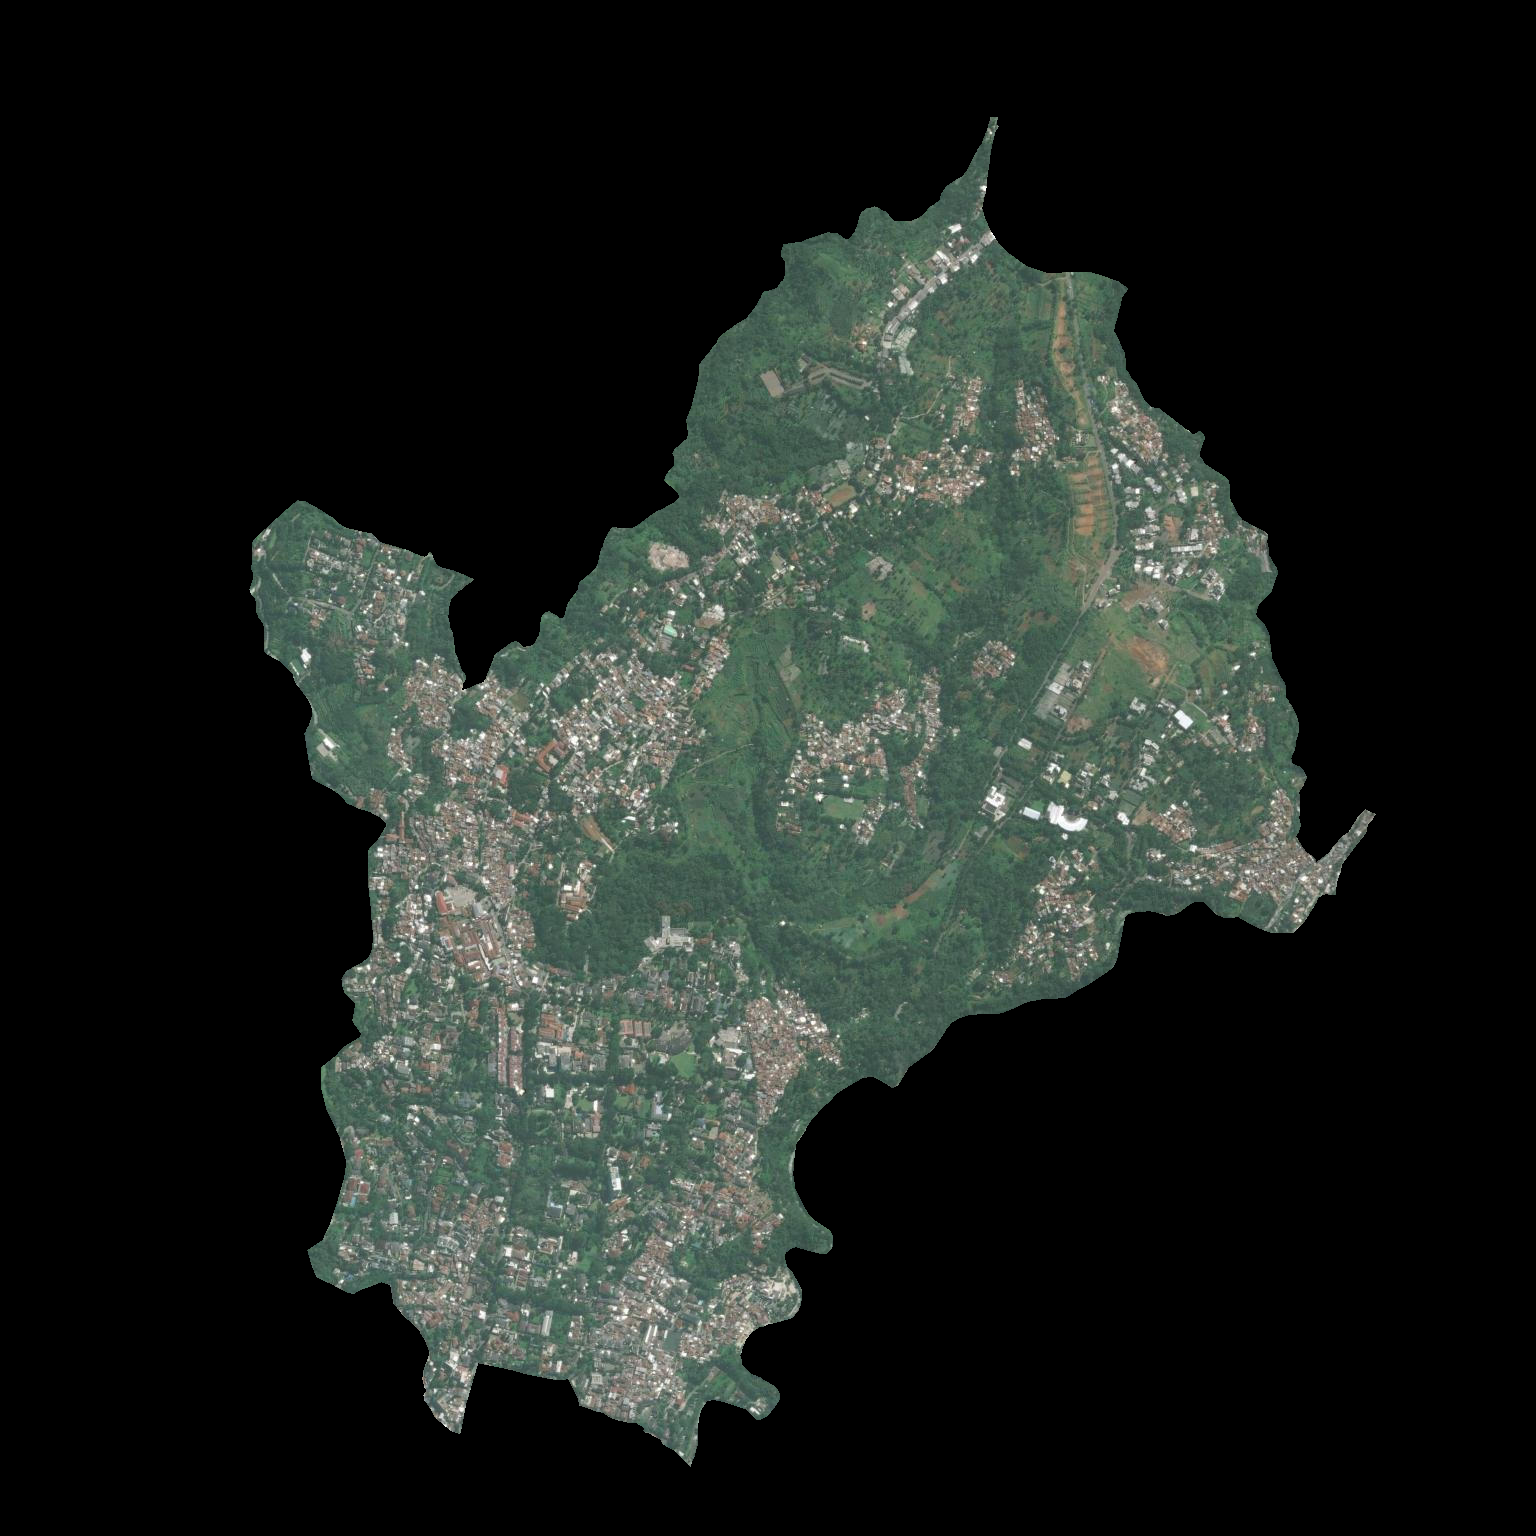
\includegraphics[width=0.5\textwidth]{Gambar/Ciumbuleuit.png}
	\caption{Gambar seluruh tile dari kelurahan Ciumbuleuit}
	\label{fig:ciumbuleuit}
\end{figure} 

Pertama-tama data yang diambil dari sistem Hadoop yang disimpan pada Hadoop Laboratoium Unpar. Kemudian data yang telah diambil berupa file ".txt" yang setiap baris dari file tersebut merupakan sebuah file gambar berupa \textit{tile} seperti pada gambar(\ref{fig:tileCiumbuleuit}). Kumpulan gambar per \textit{tile} akan digabungkan dengan menggunakan \textit{script}. Penggabungan gambar setiap \textit{tile} akan menghasilkan sebuah gambar dari kecamatan/kelurahan seperti pada gambar \ref{fig:ciumbuleuit}.
\begin{figure}[H]
	\centering
	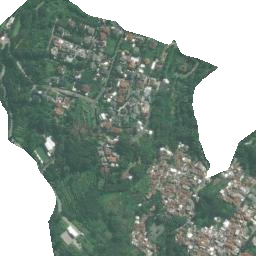
\includegraphics[scale=0.4]{Ciumbuleuit21.png}
	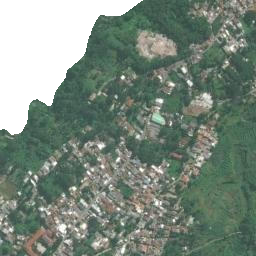
\includegraphics[scale=0.4]{Ciumbuleuit22.png}
	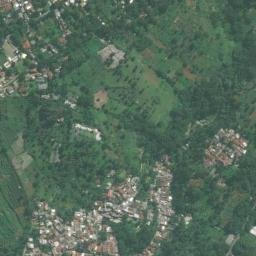
\includegraphics[scale=0.4]{Ciumbuleuit23.png}
	\caption{Contoh gambar kelurahan Ciumbuleuit setiap \textit{tile}}
	\label{fig:tileCiumbuleuit}
\end{figure}

\subsection{Mengunduh File Text}

Pada penelitian yang telah dilakukan oleh Juan Anthonius Kusjadi menghasilkan data yang telah disimpan pada sistem \textit{data lake }yang telah dibuat pada Hadoop
HDFS.\cite{juan:22:pengumpulan} Pada proses pengunduhan data harus terlebih dahulu mendaftarkan akun HDFS pada admin laboratoium FTIS UNPAR(Universitas Katholik Parahyangan) agar mendapat akses kedalam sistem penyimpanan HDFS(\textit{Hadoop Distributed File System}). Setelah mendapatkan aksesnya, lalu dapat mengunduh data citra satelit kelurahan per kota dengan perintah seperti pada kode \ref{code:cmdhdfs}. 

\begin{lstlisting}[language=Bash, caption=\textit{Command-line} HDFS,label={code:cmdhdfs}]
	>hdfs dfs -get /user/if18059/geodata/cropped/arcgis/16/Jawa_Barat/Kota_Bandung.txt .	
\end{lstlisting}


Metode yang umum digunakan untuk mengunduh file dari server jarak jauh secara aman adalah dengan menggunakan SCP (\textit{Secure Copy Protocol}). SCP adalah perintah baris perintah yang memungkinkan pengguna untuk mentransfer file antara komputer lokal dan server jarak jauh melalui koneksi yang aman. Dalam pengunduhan file dari server dapat menggunakan perintah 'scp' diikuti oleh alamat sumber file di server dan alamat tujuan pada penyimpanan lokal. Dapat dilihat pada \textit{command-line} \ref{code:cmdscp}, akan mengunduh file 'Kota\_Bandung.txt' dari server HDFS laboratorium FTIS UNPAR ke lokasi yang ditentukan pada penyimpanan lokal. Dengan demikian, File yang telah diunduh dapat dengan mudah digunakan.

\begin{lstlisting}[language=Bash, caption=\textit{Command-line} SCP,label={code:cmdscp}]
	C:\Users\Asus>scp ssh i17086@10.100.69.101:Kota_Bandung.txt	
\end{lstlisting}

Data Kota\_Bandung.txt dapat dilihat pada gambar \ref{fig:kotabandungteks}. Isi dari berkas Kota\_Bandung.txt memiliki 9 kolom yang dipisahkan oleh tanda titik koma (”;”). Pada kolom pertama diisi dengan nama kelurahan. Pada kolom kedua diisi dengan nama kota. Pada kolom ketiga diisi dengan nama provinsi. Kolom keempat diisi dengan nilai panjang tile untuk kelurahan tersebut. Kolom kelima diisi dengan nilai lebar dari tile untuk kelurahan tersebut. Kolom keenam diisi dengan posisi x koordinat tile untuk kelurahan tersebut. Kolom ketujuh diisi dengan posisi y koordinat tile untuk kelurahan tersebut. Kolom kedelapan diisi dengan ukuran luas per piksel dalam km2 untuk tile pada kelurahan tersebut. Terakhir kolom kesembilan diisi dengan data
tile citra satelit dengan format png yang sudah dienkripsi dalam bentuk Base64.\cite{juan:22:pengumpulan}
 

\begin{figure}[H]
	\centering
	\includegraphics[width=0.8\textwidth]{Gambar/data kota\_bandung.png}
	\caption{Data Citra Satelit berupa .txt}
	\label{fig:kotabandungteks}
\end{figure} 

\subsection{Mengkonversi Baris Menjadi Gambar .png}
\label{subsec:pengkorvesianBaris}
Dalam penelitian ini, telah dikembangkan sebuah \textit{script} yang bertujuan untuk mengekstraksi gambar pertile dari data Kota\_Bandung.txt. Script yang telah dikembangkan dapat dilihat kode program \ref{code:ekstraksiGambar}.

\begin{lstlisting}[language=Python, caption=Script Mengekstrasi gambar per tile,label={code:ekstraksiGambar}]
	import base64
	
	file = open("Kota_Bandung.txt","r+")
	kordinat_x = 0
	kordinat_y = 0
	result = []
	
	for line in file:
		file_line = file.readline().split(";",8)   
		image_data = file_line[8]
		kordinat_x = file_line[5]
		kordinat_y = file_line[6]
		
		
		imgdata = base64.b64decode(image_data)
		filename = file_line[0] + str(kordinat_x) + str(kordinat_y)+ '.png'
		with open(filename,'wb') as imgd:
		imgd.write(imgdata)
	
	file.close()
		
\end{lstlisting}

\textit{Script }ini menggunakan \textit{library} base64 untuk mengelola data gambar yang disimpan dalam format base64. Pertama, \textit{script} membuka file Kota\_Bandung.txt dalam mode pembacaan ('r+'). Variabel kordinat\_x dan kordinat\_y diinisialisasi ke nilai 0. Selama iterasi berlangsung, data dari file dibaca per baris menggunakan perulangan \textit{for line in file}. Setiap baris diproses dengan membaginya menjadi elemen-elemen dengan pemisah titik koma (';'). Data gambar yang terdapat di kolom ke-8 di-\textit{decode} dari format base64 menggunakan base64.b64decode dan disimpan dalam variabel imgdata. Selanjutnya, nama file gambar ditentukan dengan menggabungkan beberapa elemen, seperti nama kecamatan atau kelurahan, kordinat\_x, dan kordinat\_y, dan diberi ekstensi '.png'.

Gambar yang telah di-decode dan disimpan dalam imgdata lalu ditulis ke dalam file baru dengan nama yang telah ditentukan dalam mode binary ('wb') menggunakan \textit{open} dan imgd.write. Terakhir, setelah selesai mengolah semua baris, file sumber Kota\_Bandung.txt ditutup menggunakan \textit{file.close()}. Dengan \textit{script} code ini, data gambar dalam format base64 di-\textit{extract} dan disimpan sebagai file gambar .png dengan nama yang koordinat\_x dan koordinat\_y. Hasil dari penkonversian gambar dari bari dapat dilihat pada \ref{fig:pertileciumbuleuit}

\begin{figure}[H]
	\centering
	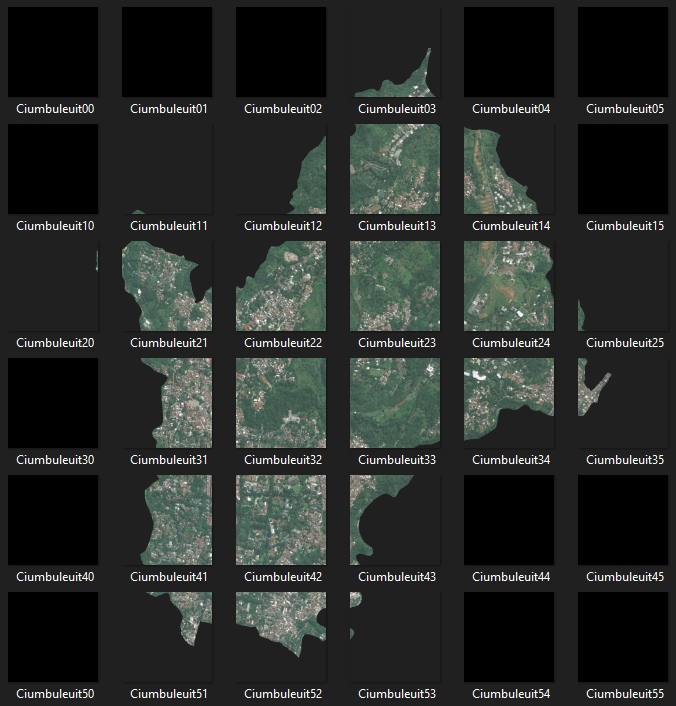
\includegraphics[width=0.5\textwidth]{Gambar/result gambar per tile.png}
	\caption{Gambar seluruh tile dari kelurahan Ciumbuleuit}
	\label{fig:pertileciumbuleuit}
\end{figure} 

\subsection{Menggabungkan Gambar}
\label{subsec:gabunggambar}
\textit{Script} yang dikembangkan dalam penelitian ini memiliki tujuan utama untuk menggabungkan sejumlah gambar per tile menjadi sebuah gambar utuh yang merepresentasikan kelurahan atau kecamatan. Kode pemrograman dapat dilihat pada kode program \ref{code:penggabunganGambar}, menggunakan library PIL (\textit{Python Imaging Library}) dengan mengimpor kelas \textit{Image}. Terdapat beberapa variabel kunci yang ditentukan, seperti nama\_kecamatan, jumlah\_baris, dan jumlah\_kolom, yang digunakan untuk mengidentifikasi nama kecamatan atau kelurahan serta jumlah baris dan kolom yang digunakan untuk mengatur tata letak gambar per tile.

\begin{lstlisting}[language=Python, caption=Script Penggabungan Gambar,label={code:penggabunganGambar}]
	from PIL import Image
	
	nama_kecematan = 'nama_kecamatan/kelurahan'
	jumlah_baris = 2
	jumlah_kolom = 3
	
	panjang_tile = 256
	lebar_tile = 256
	
	panjang_gambar = jumlah_kolom*panjang_tile
	lebar_gambar = jumlah_baris*lebar_tile
	
	canvas = Image.new("RGB", (panjang_gambar,lebar_gambar))
	for y in range(jumlah_baris):
	for x in range(jumlah_kolom):
	img = Image.open(nama_kecematan + str(y) + str(x) +".png")
	canvas.paste(img, (x*panjang_tile,y*lebar_tile))
	canvas.save(nama_kecematan + ".png")
	
\end{lstlisting}

Selanjutnya, variabel panjang\_tile dan lebar\_tile menentukan ukuran tile, yang dalam contoh ini adalah 256 piksel. Variabel panjang\_gambar dan lebar\_gambar dihitung berdasarkan jumlah kolom dan baris, sehingga ukuran gambar akhir dapat ditentukan. Proses pembuatan gambar  dimulai dengan inisiasi variabel canvas menggunakan fungsi \textit{Image.new }dengan mode "RGB" dan ukuran gambar sesuai dengan panjang\_gambar dan lebar\_gambar. Selanjutnya, terdapat dua \textit{loop} di mana \textit{loop} pertama digunakan untuk mengatur koordinat y, dan loop kedua untuk koordinat x. Di dalam \textit{loop-loop} tersebut, variabel img digunakan untuk membuka gambar tile yang sesuai dengan koordinatnya dengan menambahkan format file yang sesuai. Gambar yang diakses melalui variabel img kemudian disisipkan ke dalam gambar utuh \textit{canvas} menggunakan fungsi \textit{paste}. Dan terakhir, \textit{canvas.save} untuk menyimpan hasil gambar akhir dengan nama sesuai dengan 'nama\_kecamatan'. Hasil akhir gambar-gambar per tile menjadi gambar utuh yang merepresentasikan wilayah atau kecamatan yang diinginkan seperti pada gambar \ref{fig:ciumbuleuit}.

\section{Pembentukan Gambar Hasil Segmentasi/Klasterisasi}
Pada penelitian yang telah dilakukan oleh Juan Anthonius Kusjadi menghasilkan data hasil segmentasi area hijau yang telah disimpan pada sistem \textit{data lake }yang telah dibuat pada Hadoop
HDFS.\cite{juan:22:pengumpulan} Pengunduhan data gambar citra satelit hasil segmentasi area hijau kelurahan dapat dilakukan dengan kode perintah seperti pada kode \ref{code:cmdhdfssegmentasi}

\begin{lstlisting}[language=Bash, caption= Pengembailan Data Hasil Segemntasi,label={code:cmdhdfssegmentasi}]
	>hdfs dfs -get /user/if18059/geodata/result/kmeans-5/arcgis/16/Jawa_Barat/Kota_Bandung.csv .	
\end{lstlisting}

Kode Perintah \ref{code:cmdhdfssegmentasi} digunakan untuk mengunduh file CSV dari HDFS dan menyimpannya di direktori lokal tempat menjalankan perintah tersebut. Perintah \texttt{hdfs dfs -get} merupakan perintah untuk mengunduh file dari HDFS. Perintah /user/if18059/geodata/result/kmeans-5~~/arcgis/16/Jawa\_Barat/Kota\_Bandung.csv adalah jalur lengkap ke file yang ingin diunduh dari HDFS. File yang dimaksud adalah \texttt{Kota\_Bandung.csv} yang terletak di direktori /user/if18059/geodata/result/\\kmeans-5/arcgis/16/Jawa\_Barat/ di HDFS. Dan Perintah titik ("\texttt{.}") merupakan tempat menyimpan file yang diunduh ke direktori lokal.
	

File Kota\_Bandung.csv berisikan data hasil klasterisasi. Isi dari file Kota\_Bandung.csv memiliki 9 kolom yang dipisahkan oleh tanda titik koma (”;”). Pada kolom pertama diisi dengan nama kelurahan. Pada kolom kedua diisi dengan posisi x tile citra satelit. Pada kolom ketiga diisi dengan posisi y tile citra satelit. Pada kolom keempat diisi dengan nilai panjang dari tile citra satelit pada kelurahan tersebut. Pada kolom kelima diisi dengan nilai lebar dari tile citra satelit pada kelurahan tersebut. Pada kolom keenam diisi dengan data gambar citra satelit yang sudah disegmentasi dengan format png berdasarkan hasil klasterisasi dan di enkripsi menggunakan Base64. Pada kolom ketujuh diisi dengan data gambar citra satelit asli dengan format png dan di enkripsi menggunakan Base64. Pada kolom kedelapan diisi dengan nilai luas area hijau dalam km2. Terakhir pada kolom kesembilan diisi dengan nilai luas area kelurahan.\cite{juan:22:pengumpulan} 

Proses pengekstrasian file Kota\_Bandung.csv berbeda dengan proses pengektrasian yang ada pada \ref{subsec:pengkorvesianBaris} dikarenakan format file yang berbeda maka script yang digunakan juga berbeda. Penggunaan script dapat pada file Kota\_Bandung.csv dilihat pada \ref{code:ekstrakCSV}. 
\begin{lstlisting}[language=Python, caption=Script Penggabungan Gambar Hasil Klasterisasi ,label={code:ekstrakCSV}]
	import base64
	import csv
	
	def extract_image_pertile(csv_file):
		with open(csv_file, 'r') as file:
			csv_reader = csv.reader(file)
	
			for row in csv_reader:
				kelurahan = row[0]
				kordinat_x = row[1]
				kordinat_y = row[2]
				segmented_image_data = row[5]
				img_data = base64.b64decode(segmented_image_data)
				filename = f"{kelurahan}{kordinat_y}{kordinat_x}.png"
				
				with open(filename, 'wb') as img_file:
				img_file.write(img_data)
	
	
	if __name__ == "__main__":
	
	csv_file = "Kota_Bandung.csv"
	csv.field_size_limit(1000000)
	
	extract_image_pertile(csv_file)
	
	
\end{lstlisting}

Script Python di atas dirancang untuk memproses data gambar tersegmen dalam format base64 yang terdapat dalam sebuah file Kota\_Bandung.csv. Script ini  bertujuan untuk mengekstrak dan mendekode data gambar tersebut, kemudian menyimpannya sebagai file gambar PNG. Fungsi utama yang terlibat dalam proses ini disebut \textit{extract\_image\_pertile}, yang akan menerima nama file CSV sebagai parameter. Fungsi tersebut membuka file Kota\_Bandung.csv, lalu membaca setiap baris, dan membaca nilai-nilai yang pentin seperti kelurahan, koordinat x dan y, serta data gambar tersegmen yang dienkripsi dalam base64. Selanjutnya, data gambar tersebut didekode menggunakan \textit{library }base64 dan disimpan sebagai file gambar PNG dengan nama sesuai dengan kelurahan yang terbentuk dari gabungan nilai-nilai kolom tertentu.

Dalam bagian utama script, terdapat pemanggilan fungsi \textit{extract\_image\_pertile }dengan menyertakan nama file Kota\_Bandung.csv yang akan diproses. Sebagai tambahan, script ini mengatur batas ukuran untuk file CSV dengan csv. Fungsi \textit{field\_size\_limit} untuk menangani batasan ukuran default yang ada. Dengan menjalankan script ini, file gambar PNG akan dihasilkan untuk setiap baris. Gambar dari setiap baris tersebut merupakan gambar pertile dari tiap kelurahan.

Setelah mendapatkan gambar per tile langkah selanjut yaitu menggabungkan gambar. Proses penggabungan gambar segmentasi area hijau sama dengan proses penggabungan gambar kelurahan sebelum segmentasi. Pada proses tersebut dapat dilihat pada bab \ref{subsec:gabunggambar}.



\section{Analisis Perangkat Lunak}
Proses analisis perangkat lunak merupakan kebutuhan yang memerlukan peranan seorang pengguna untuk menjalankan sebuah perangkat lunak yang akan dikembankan. Sehingga segala proses sistem dijalankan oleh aktor yang terlibat. Dalam sistem ini hanya memiliki aktor sebagai \textit{user}. Seorang pemangku kepentingan atau pembuat keputusan memegang peranan sebagai \textit{user} itu sendiri. Dalam menggambarkan peranan pengguna terhadap interaksinya dengan sistem, maka dapat dilihat pada diagram \textit{use case} yang terdapat pada Gambar~\ref{fig:useCaseUser} berikut.

\begin{figure}[H]
	\centering
	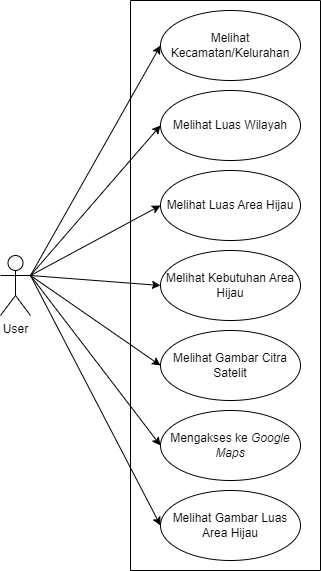
\includegraphics[scale=0.5]{Gambar/UseCaseUser.png}
	\caption[Diagram \textit{Use Case} \textit{User}]{Diagram \textit{Use Case} \textit{User}}
	\label{fig:useCaseUser}
\end{figure}

Pada Gambar~\ref{fig:useCaseUser}, seorang aktor atau \textit{user} pada sistem berperan dalam memegang akses penuh ke dalam sistem. Dalam hal ini \textit{user} dapat masuk ke dalam sistem yang telah dibangun, dapat memilih kecamatan/kelurahan yang ingin dilihat. Setiap kecamatan/kelurahan yang dipilih \textit{user} dapat melihat luas wilayah, luas area hijau, kebutuhan area hijau, gambar citra satelit/gambar luas area hijau, dan juga dapat mengakses ke halaman \textit{Google Maps} yang merujuk ke lokasi kecamatan/kelurahan yang dipilih.
	
Berdasarkan diagram \textit{use case }pada Gambar \ref{fig:useCaseUser}, berikut adalah daftar skenario unutk setiap \textit{use case:}	

\begin{enumerate}
	\item Use Case: Melihat kecamatan atau kelurahan \\
	\textit{\textbf{Actor}}: Pengguna \\
	\textit{\textbf{Pre Condition: }}Pengguna telah dapat mengakses website dan berada pada halaman utama website\\
	\textit{\textbf{Post Condition:}} Pengguna melihat infromasi dari kecamatan atau kelurahan dipilih\\
	\textit{\textbf{Steps: }}
	\begin{table}[H]
		\centering
		\resizebox{0.9\columnwidth}{!}{%
			\begin{tabular}{|l|l|}
				\hline
				\textbf{\textit{Actor Actions}}                                       & \textbf{\textit{System Response}}                                          \\ 
				\hline
				Pengguna menekan pada \textit{dropdown }kecamatan/kelurahan\textit{~} &                                                                            \\
				& \textit{Dropdown}~akan menampilkan daftar kecamatan/kelurahan              \\
				Pengguna dapat menekan salah satu pada daftar kecamatan/kelurahan     &                                                                            \\
				& Menampilkan informasi dari kecamatan/kelurahan yang dipilih oleh pengguna  \\
				\hline
			\end{tabular}%
		}
		
	\end{table}
	
	\item Use Case: Melihat luas wilayah kelurahan\\
	\textit{\textbf{Actor}}: Pengguna \\
	\textit{\textbf{Pre Condition: }}Pengguna telah dapat mengakses website dan berada pada halaman utama website\\
	\textit{\textbf{Post Condition:}} Pengguna melihat infromasi dari kecamatan atau kelurahan dipilih\\
	
	\item Use Case: Melihat luas area hijau kelurahan\\
	\textit{\textbf{Actor}}: Pengguna \\
	\textit{\textbf{Pre Condition: }}Pengguna telah dapat mengakses website dan berada pada halaman utama website\\
	\textit{\textbf{Post Condition:}} Pengguna melihat infromasi dari kecamatan atau kelurahan dipilih\\
	
	\item Use Case: Melihat kebutuhan area hijau\\
	\textit{\textbf{Actor}}: Pengguna \\
	\textit{\textbf{Pre Condition: }}Pengguna telah dapat mengakses website dan berada pada halaman utama website\\
	\textit{\textbf{Post Condition:}} Pengguna melihat infromasi dari kecamatan atau kelurahan dipilih\\
	
	\item Use Case: Melihat gambar citra satelit\\
	\textit{\textbf{Actor}}: Pengguna \\
	\textit{\textbf{Pre Condition: }}Pengguna telah dapat mengakses website dan berada pada halaman utama website\\
	\textit{\textbf{Post Condition:}} Pengguna melihat infromasi dari kecamatan atau kelurahan dipilih\\
	
	\item Use Case: Mengakses ke \textit{google maps}\\
	\textit{\textbf{Actor}}: Pengguna \\
	\textit{\textbf{Pre Condition: }}Pengguna telah dapat mengakses website dan berada pada halaman utama website\\
	\textit{\textbf{Post Condition:}} Pengguna melihat infromasi dari kecamatan atau kelurahan dipilih\\
	
	\item Use Case: Melihar gambar luas area hijau\\
	\textit{\textbf{Actor}}: Pengguna \\
	\textit{\textbf{Pre Condition: }}Pengguna telah dapat mengakses website dan berada pada halaman utama website\\
	\textit{\textbf{Post Condition:}} Pengguna melihat infromasi dari kecamatan atau kelurahan dipilih\\
\end{enumerate}



\begin{table}[H]
	\centering
	\caption{Skenario melihat kecamatan atau kelurahan}
	\label{tab:melihatKecamatanatauKelurahan}
	\resizebox{\columnwidth}{!}{%
		\begin{tabular}{|l|l|}
			\hline
			\textit{Use Case}        & Melihat kecamatan/kelurahan                                                                   \\ \hline
			Aktor                    & \textit{User}                                                                                 \\ \hline
			Tujuan                   & Melihat informasi dari kecamatan/kelurahan yang dipilih oleh user                             \\ \hline
			Kondisi                  & \textit{User} telah dapat mengakses website dan berada pada halaman utama dari website                 \\ \hline
			\multirow{4}{*}{Langkah} & 1. \textit{User} menekan pada \textit{dropdown} kecamatan/kelurahan                                             \\ \cline{2-2} 
			& 2. \textit{Dropdown} akan menampilkan daftar kecamatan/kelurahan                                       \\ \cline{2-2} 
			& 3. \textit{User} dapat menekan salah satu pada daftar kecamatan/kelurahan                              \\ \cline{2-2} 
			& 4. Perangkat lunak akan menampilkan informasi dari kecamatan/kelurahan yang dipilih oleh \textit{user} \\ \hline
		\end{tabular}%
	}
\end{table}

\begin{table}[H]
	\centering
	\caption{Skenario melihat luas wilayah kecamatan/kelurahan}
	\label{tab:melihatLuasWilayah}
	\resizebox{\columnwidth}{!}{%
		\begin{tabular}{|l|l|}
			\hline
			\textit{Use Case} & Melihat kebutuhan area hijau                                                                       \\ \hline
			Aktor             & \textit{User}                                                                                      \\ \hline
			Tujuan            & Melihat kebutuhan area hijau dari kecamatan/kelurahan yang dipilih                                 \\ \hline
			Kondisi           & \textit{User} berada pada halaman utama dari website dan telah milih kecamatan/kelurahan yang ingin dilihat \\ \hline
			Langkah           & 1. Perangkat Lunak akan menampilkan kebutuhan area hijau dari kecamatan/kelurahan yang dipilih     \\ \hline
		\end{tabular}%
	}
\end{table}

\begin{table}[H]
	\centering
	\caption{Skenario melihat luas area hijau}
	\label{tab:melihatLuasAreaHijau}
	\resizebox{\columnwidth}{!}{%
		\begin{tabular}{|l|l|}
			\hline
			\textit{Use Case} & Melihat luas area hijau                                                                       \\ \hline
			Aktor             & \textit{User}                                                                                      \\ \hline
			Tujuan            & Melihat luas area hijau dari kecamatan/kelurahan yang dipilih                                 \\ \hline
			Kondisi           & \textit{User} berada pada halaman utama dari website dan telah milih kecamatan/kelurahan yang ingin dilihat \\ \hline
			Langkah           & 1. Perangkat Lunak akan menampilkan luas area hijau dari kecamatan/kelurahan yang dipilih     \\ \hline
		\end{tabular}%
	}
\end{table}

\begin{table}[H]
	\centering
	\caption{Skenario melihat kebutuhan area hijau}
	\label{tab:melihatKebutuhanAreaHijau}
	\resizebox{\columnwidth}{!}{%
		\begin{tabular}{|l|l|}
			\hline
			\textit{Use Case} & Melihat kebutuhan area hijau                                                                       \\ \hline
			Aktor             & \textit{User}                                                                                      \\ \hline
			Tujuan            & Melihat kebutuhan area hijau dari kecamatan/kelurahan yang dipilih                                 \\ \hline
			Kondisi           & \textit{User }berada pada halaman utama dari website dan telah milih kecamatan/kelurahan yang ingin dilihat \\ \hline
			Langkah           & 1. Perangkat Lunak akan menampilkan kebutuhan area hijau dari kecamatan/kelurahan yang dipilih     \\ \hline
		\end{tabular}%
	}
\end{table}

\begin{table}[H]
	\centering
	\caption[Skenario melihat gambar citra satelit]{Skenario melihat gambar citra satelit}
	\resizebox{\columnwidth}{!}{%
		\begin{tabular}{|l|l|}
			\hline
			\textit{Use Case} & Melihat gambar citra satelit                                                                       \\ \hline
			Aktor             & \textit{User}                                                                                      \\ \hline
			Tujuan            & Melihat gambar citra satelit dari kecamatan/kelurahan yang dipilih                                 \\ \hline
			Kondisi           & \textit{User} berada pada halaman utama dari website dan telah milih kecamatan/kelurahan yang ingin dilihat \\ \hline
			Langkah           & 1. Perangkat Lunak akan menampilkan gambar citra satelit dari kecamatan/kelurahan yang dipilih     \\ \hline
		\end{tabular}%
	}
\end{table}

\begin{table}[H]
	\centering
	\caption{Skenario mengakses ke google maps}
	\label{tab:mengakseskegooglemaps}
	\resizebox{\columnwidth}{!}{%
		\begin{tabular}{|l|l|}
			\hline
			\textit{Use Case}        & Mengakses ke Google Maps                                                                           \\ \hline
			Aktor                    & \textit{User}                                                                                      \\ \hline
			Tujuan                   & Mengakses \textit{Google Maps }dari kecamatan/kelurahan yang dipilih                                        \\ \hline
			Kondisi                  & \textit{User }berada pada halaman utama dari website dan telah milih kecamatan/kelurahan yang ingin dilihat \\ \hline
			\multirow{3}{*}{Langkah} & 1. Perangkat Lunak akan menampilkan link google maps dari kecamatan/kelurahan yang dipilih         \\ \cline{2-2} 
			& 2. User menekan link yang ditampilkan                                                              \\ \cline{2-2} 
			& 3. User akan diarahkan ke halaman \textit{Google Maps}                                             \\ \hline
		\end{tabular}%
	}
\end{table}


\begin{table}[H]
	\centering
	\caption{Skenario melihat gambar luas area hijau}
	\label{tab:melihatgambarareahijau}
	\resizebox{\columnwidth}{!}{%
		\begin{tabular}{|l|l|}
			\hline
			\textit{Use Case} & Melihat gambar luas area hijau                                                                     \\ \hline
			Aktor             & \textit{User}                                                                                      \\ \hline
			Tujuan            & Meliuhat gambar luas area hijau dari kecamatan/kelurahan yang dipilih                              \\ \hline
			Kondisi           & \textit{User} berada pada halaman utama dari website dan telah milih kecamatan/kelurahan yang ingin dilihat \\ \hline
			Langkah           & 1. Perangkat Lunak akan gambar citra satelit dari kecamatan/kelurahan yang dipilih                 \\ \hline
			& 2. \textit{User} menekan \textit{radio button} area hijau                                                            \\ \hline
			& 3. Perangkat Lunak akan gambar luas area hijau dari kecamatan/kelurahan yang dipilih               \\ \hline
		\end{tabular}%
	}
\end{table}